\documentclass{article}
\usepackage[widepage]{repsty}

\newcommand{\y}{\mathbf{y}}

\usepgfplotslibrary{fillbetween}


\begin{document}

The probability of observing  the value $y_i \equiv y(t_i)$ when the expectation value is $\mu(t_i)$ and the error is Gaussian is
\begin{align*}
	f(y_i|\pars) &= \frac{1}{\sqrt{2\pi\nu}}\exp\bkt{-\frac12\frac{(y_i - \mu(t_i))^2}{\nu}}, \\
	\pars 		  &= (\nu,\omega,\phi),\\
	\mu(t_i) 	  &= N_0\bkt{1 + P\sin(\omega t_i + \phi)}.
\end{align*}

The likelihood of observing a set of observations $\y = (y_1,\dots, y_K)$, under the i.i.d. assumption, is the product of propabilities taken as a function of the parameters:
\begin{align*}
	\mathcal{L}(\pars|\y) &= \prod_i f(y_i|\pars),
\shortintertext{and the log-likelihood}
	\ell(\pars|\y) &= -\frac{K}{2}\log2\pi - \frac{K}{2}\log\nu - \frac{1}{2\nu}\sum_i\epsilon_i^2,
	~ \epsilon_i = y_i- \mu(t_i).
\end{align*}
The usual assumptions for the error term are zero expectation and strict exogeneity
\begin{align*}
	\XpctO{\epsilon_i} &= \XpctO{t_i\epsilon_i} = 0,
\intertext{and the relations between the mean's derivatives are}
	\mu'_\phi	&= N_0P\cos(\omega t + \phi), \\
	\mu'_\omega &= t\cdot\mu'_\phi, \epsilon'_\xi = -\mu'_\xi.
\end{align*}

The log-likelihood derivatives:
\begin{align*}
\ell'_\nu 		&= -\frac{K}{2\nu} + \frac{1}{2\nu^2}\sum_i\epsilon_i^2;  & \\
\ell'_\omega 	&= \frac1\nu\sum_i\mupp t_i\epsilon_i;  & \\
\ell'_\phi		&= \frac1\nu \sum_i \mupp\epsilon_i; & \\
%
\ell''_{\nu^2}		&= \frac{K}{2\nu^2} - \frac{1}{\nu^3}\sum_i\epsilon_i^2, 
	&-\XpctO{\ell''_{\nu^2}} = \frac{K}{2\nu^2} - \frac{1}{\nu^3}\sum_i\nu = \frac{K}{2\nu^2};\\
\ell''_{\nu\omega}	&= -\frac{1}{\nu^2}\sum_i\mupp t_i\epsilon_i, 
	&-\XpctO{\ell''_{\nu\omega}} = \frac{1}{\nu^2}\sum_i\mupp\XpctO{t_i\epsilon_i} = 0;\\
\ell''_{\nu\phi}	&= -\frac{1}{\nu^2}\sum_i\mupp \epsilon_i, 
	&-\XpctO{\ell''_{\nu\phi}} = \frac{1}{\nu^2}\sum_i\mupp\XpctO{\epsilon_i} = 0; \\
\ell''_{\phi^2}		&= \frac1\nu\sum_i\bkt{\mudpp \epsilon_i - \bkt{\mupp}^2}, 
	&-\XpctO{\ell''_{\phi^2}} = \frac1\nu\sum_i\bkt{\bkt{\mupp}^2 - \mudpp\XpctO{\epsilon_i}} = \frac1\nu\sum_i\bkt{\mupp}^2;\\
\ell''_{\phi\omega}	&= \frac1\nu\sum_i\bkt{\mudpp t_i\epsilon_i - \bkt{\mupp}^2t_i}, 
	&-\XpctO{\ell''_{\phi\omega}} = \frac1\nu\sum_i\bkt{t_i\bkt{\mupp}^2 - \mudpp\XpctO{t_i\epsilon_i}} = \frac1\nu\sum_i t_i\bkt{\mupp}^2;\\
\ell''_{\omega^2}	&= \frac1\nu\sum_i\bkt{\mudpp t_i^2\epsilon_i - \bkt{\mupp t_i}^2},
	& -\XpctO{\ell''_{\omega^2}} = \frac1\nu\sum_i\bkt{\bkt{t_i\mupp}^2 - \mudpp\XpctO{t_i^2\epsilon_i}} = \frac1\nu\sum_i\bkt{t_i\mupp}^2.
\end{align*}

\section{Variances}

The Fisher matrix
\[
	\Fisher = \begin{pmatrix}
	\sfrac{K}{2\nu} & 0 								& 0 \\
	0 				& \sfrac1\nu\sum\bkt{t_i\mupp}^2	& \sfrac1\nu\sum t_i\bkt{\mupp}^2 \\
	0				& \sfrac1\nu\sum t_i\bkt{\mupp}^2	&\sfrac1\nu\sum\bkt{\mupp}^2
	\end{pmatrix}.
\]
The determinant
\newcommand{\STM}{\Omega}
\[
	|\Fisher| = \frac{K}{2\nu^3}\underbrace{\bkt{\sum\bkt{t_i\mupp}^2\sum\bkt{\mupp}^2 - \bkt{\sum t_i\bkt{\mupp}^2}^2}}_{\STM}.
\]
The variance-covariance matrix
\[
vcov = \begin{pmatrix}
	\sfrac{2\nu}{K}& 0									& 0				\\
	0				&\nu\frac{\sum\bkt{\mupp}^2}{\STM}		&\nu\frac{\sum t_i\bkt{\mupp}^2}{\STM}\\
	0				&\nu\frac{\sum t_i\bkt{\mupp}^2}{\STM}	&\nu\frac{\sum\bkt{t_i\mupp}^2}{\STM}
\end{pmatrix}.
\]

The variance of the frequency estimate
\begin{equation}\label{eq:Var1}
	\var{\hat{\omega}} = \nu\frac{\sum\bkt{\mupp}^2}{\sum\bkt{t_i\mupp}^2\sum\bkt{\mupp}^2 - \bkt{\sum t_i\bkt{\mupp}^2}^2}.
\end{equation}

\paragraph{Cross-check.} Let $\mu(t_i) = \phi + \omega t_i$. In that case $\mupp = 1$, $\mu'_\omega(t_i) = t_i = t_i\cdot\mupp$, the determinant of the Fisher matrix simplifies to 
\begin{align*}
	|\Fisher| &= \frac{K}{2\nu^4}\bkt{K\sum_i t_i^2 - \bkt{\sum t_i}^2} \\
				 &= \frac{K^3}{2\nu^4}\bkt{\frac1K\sum t_i^2 - \avg{t}^2} \\
				 &= \frac{K}{2\nu^4}\cdot\underbrace{K\sum\bkt{t_i - \avg{t}}^2}_{\STM}
\end{align*}
\newcommand{\SSX}{\sum\bkt{t_i - \avg{t}}^2}
and the variance-covariance matrix becomes
\[
vcov = \begin{pmatrix}
	2\sfrac{\nu^2}{K}& 0									& 0				\\
	0				&\frac{\nu}{\SSX}		&\nu\frac{\sum t_i}{K\SSX}\\
	0				&\nu\frac{\sum t_i}{K\SSX}	&\nu\frac{\sum t_i^2}{K\SSX}
\end{pmatrix},
\]
with the well-known expression for the slope variance
\[
	\var{\hat\omega} = \frac{\nu}{\SSX}.
\]

Let us denote $\bkt{\mupp}^2 = (N_0P)^2\cos^2(\omega t_i + \phi) \equiv x_i$. Eq.~\eqref{eq:Var1} can be rewritten in the following form:
\begin{align}
\var{\hat\omega} &= \frac{\nu}{\sum_j x_j \bkt{\sum_i t_i^2 \frac{x_i}{\sum_j x_j} - \bkt{\sum_i t_i \frac{x_i}{\sum_j x_j}}^2}} \notag\\
				&= \frac{\nu}{\sum_j x_j \sum_i w_i\bkt{t_i - \avg{t}[w]}^2} \notag\\
				&= \frac{\nu}{\sum_j x_j \cdot\var[w]{t}}. \label{eq:Var2}
\end{align}

\newcommand{\M}{\underline{\mathrm{M}}}
\newcommand{\T}{\underline{\mathrm{T}}}
\newcommand{\diag}[1]{\mathcal{D}_{#1}}
\newcommand{\diagM}{\diag{\mu}}
In matrix form, the frequency variance is written as
\begin{align*}
\var{\hat\omega} &= \frac{\nu}{\bkt{\T'\diagM^2\T} - \bkt{\T'\diagM\M}^2/\bkt{\M'\M}}, 
\shortintertext{with}
\T &= \bkt{t_0,\dots, t_{K-1}}', ~ \M = \bkt{\mupp*(t_0),\dots,\mupp*(t_{K-1})}', \\
\diagM &= \begin{pmatrix}
	\mupp*(t_0) & 0				& \cdots & 0 \\
	0			& \mupp*(t_1)	& \cdots & 0 \\
	\vdots		& \cdots		&\ddots	 & \vdots \\
	0			& 0				&\cdots  & \mupp*(t_{K-1})
\end{pmatrix}.
\end{align*}

\section{Sampling modulation}
Suppose we write the Fisher matrix as a sum:
\begin{equation}\label{eq:FisherSum}
	\Fisher = \sum_i \Fisher[i]; 
	~\Fisher[i] = \frac1\nu\begin{pmatrix}
	\bkt{\sqrt2\cdot\mupp}^{-2} & 0 		& 0 \\
	0		 & t_i^2 	& t_i \\
	0		 &	t_i	    & 1
	\end{pmatrix}\cdot\bkt{\mupp}^2.
\end{equation}

$\Fisher[i] = -\XpctO{\frac{\partial^2}{\partial\pars^2}\log f(y_i|\pars)\vert_{\pars=\pars_0}}$ could be\footnote{The $t_i$ in the structural matrix in eq.~\eqref{eq:FisherSum} worries me, because it appears that a point carries more information simply by virtue of it being measured later in time; but as far as I can tell the reason for it is that it is assumed that the point labeled as $i$ is the $i$-th point in a series, and so a later point is more informative than a point closer to the origin, all other things being equal. And it's nothing new; in linear regression we also want our predictors to be as spread out as possible.} interpreted as the information about the parameter that's carried in $y_i$.
\begin{figure}[h]
\centering
\begin{subfigure}{.5\textwidth}
\begin{tikzpicture}
	  \draw[->] (-1.5,0) -- (1.5,0) node[right] {$\mupp$};
      \draw[->] (0,-.5) -- (0, 2.3) node[above] {$I_i(\pars_0)$};
      \draw[scale=1,domain=-1.5:1.5,smooth,variable=\x,red] plot ({\x},{\x*\x});
\end{tikzpicture}
\caption{Fisher information of a point is a parabola of the signal derivative.}
\end{subfigure}~
\begin{subfigure}{.5\textwidth}
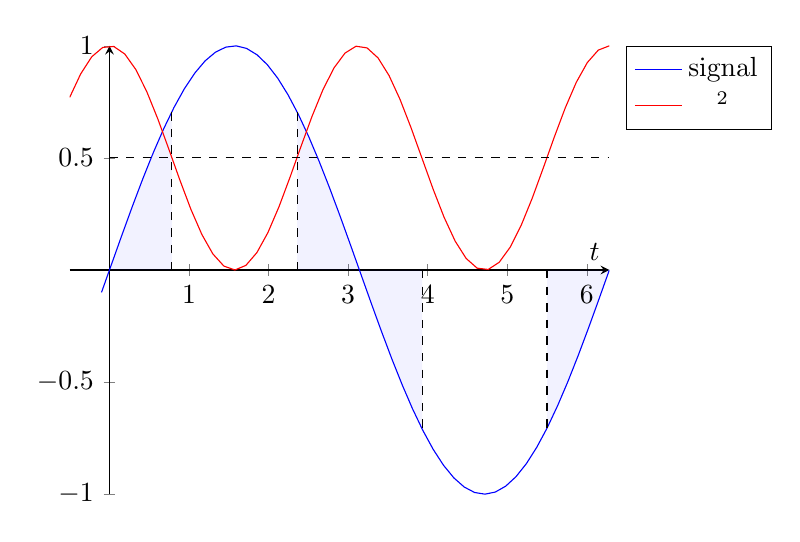
\begin{tikzpicture}
\begin{axis}[axis lines=center, xlabel=$t$, domain=-.5:2*pi, legend pos=outer north east]
	\addplot[color=blue, name path=signal, domain=-.1:2*pi,samples=50] {sin(deg(x))}; \addlegendentry{signal}
	\addplot[color=red, samples=50] {cos(deg(x))^2}; \addlegendentry{$\bkt{\mupp}^2$}
	\addplot[mark=none,dashed, domain=0:2*pi]{.5};
	\draw[dashed] (axis cs:.785,0) -- (axis cs:.785,{sin(deg(.785))});
	\draw[dashed] (axis cs:2.36,0) -- (axis cs:2.36,{sin(deg(2.36))});
	\draw[dashed] (axis cs:3.93,0) -- (axis cs:3.93,{sin(deg(3.93))});
	\draw[dashed] (axis cs:5.5,0) -- (axis cs:5.5,{sin(deg(5.5))});
	\path[name path=axis] (axis cs:0,0) -- (axis cs:2*pi,0);
	\addplot[fill=blue, opacity=.05] fill between [of=signal and axis, soft clip={domain=0:.785}];
	\addplot[fill=blue, opacity=.05] fill between [of=signal and axis, soft clip={domain=2.36:3.93}];
	\addplot[fill=blue, opacity=.05] fill between [of=signal and axis, soft clip={domain=5.5:2*pi}];
\end{axis}     
\end{tikzpicture}
\caption{Filled areas are where the points are more informative.}
\end{subfigure}
\end{figure}

If we attribute each point a weight proportional to its Fisher information, i.e. $w_i = \cos^2(\omega t_i + \phi)$,~\footnote{The variance of $\omega$ is proportional to the (2,2)-minor, in which time doesn't figure, only the squared cosine.} the weight of a region where $\bkt{\mupp}^2 \geq\sfrac12$ is greater than that of an equivalent region with $\bkt{\mupp}^2 < \sfrac12$  by the factor:
\begin{align*}
	\int_{t_0}^{t_1}\cos^2(\omega t + \phi)\td t = \frac1\omega\int_{\omega t_0}^{\omega t_1} \cos^2\theta\td\theta = \frac{\Delta t}{2} + \frac{1}{2\omega}\sin\omega\Delta t\cos\omega\Sigma t \approx 1.9.
\end{align*}

The implication is that increasing the number of points measured during the signal's rise and fall is roughly twice as beneficial as doing so during the peaks and troughs.

%\section{The dependence of $\var{\hat{\omega}}$ on $\omega$}
%\newcommand{\acos}{\mathrm{acos}}
%The variance in eq.~\eqref{eq:Var2} is conditional on the frequency $\omega$ and phase $\phi$ of the signal. The conditioning happens because the parameters determine the sampling range of the distribution of the $x_i$ weights.
%
%That distribution is 
%\[
%	f(x_i) = \frac{1}{\pi}\cdot\bkt*{\frac{x_i}{N_0P}\bkt{1-\frac{x_i}{N_0P}}}^{-\sfrac12}.
%\]
%
%\begin{align*}
%\Xpct{\sum_i x_i}[(\omega,\phi)] &= \sum_i \int_{\cos^2\phi}^{\cos^2(\omega t_i + \phi)}x_if(x_i)\td x_i;
%\end{align*}


\end{document}
